\section{Le modèle MVC et l'environnement Java EE}

%%%%%%%%%%%%%%%%%%%%%%%%%%%%%%%%%%%%%%%%%%%%%%%%%%%%%%%%%%
%----------------------MVC-------------------------------%
%%%%%%%%%%%%%%%%%%%%%%%%%%%%%%%%%%%%%%%%%%%%%%%%%%%%%%%%%%
\subsection{Architecture Modèle-Vue-Contrôleur}
Etant donné le fait que nous avons choisi de faire une application interactive, nous avons utilisé l'architecture logicielle \textbf{MVC}. Ainsi, les problématiques liées aux composantes de notre application sont bien séparées :
\begin{description}
 \item[Le modèle :] notre code Java qui modélise les données et qui sera relié à une base de données pour stocker diverses informations. C'est le coeur du programme.
 \item[La vue :] l'interface homme-machine qui sera sous forme d'un site Web.
 \item[Le contrôleur :] la partie de notre code qui fait le lien entre le modèle et la vue. Il agit en fonction de ce que l'utilisateur demande à la vue. Il est chargé de de chaque côté et les transmets à l'un et l'autre comme le montre le schéma ci-dessous.\\
\end{description}

Le schéma suivant présente les intéractions entre les trois entités de notre architecture logicielle.
\begin{figure}[H]
  \center
  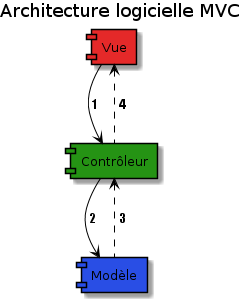
\includegraphics[scale=0.6]{../graph/MVC.png} \\
  \caption{Structure MVC}
\end{figure}

\begin{enumerate}
 \item L'utilisateur intéragi avec la vue (le site Web) et lance une action du contrôleur qui reçoit les informations.
 \item Le contrôleur agit alors en conséquence en envoyant des informations au modèle.
 \item Le modèle traite les informations puis renvoie le résultat de son action au contrôleur et des données dans certains cas.
 \item Le contrôleur fait un compte rendu à l'utilisateur en mettant à jour la vue.
\end{enumerate}

Nous allons voir dans la partie suivante comment sont implémentées nos différentes composantes.

%%%%%%%%%%%%%%%%%%%%%%%%%%%%%%%%%%%%%%%%%%%%%%%%%%%%%%%%%%
%----------------------JEE-------------------------------%
%%%%%%%%%%%%%%%%%%%%%%%%%%%%%%%%%%%%%%%%%%%%%%%%%%%%%%%%%%
\subsection{Environnement Java EE}
\subsubsection{Présentation}
L'environnement de développement Java EE (Java Enterprise Edition) est une extension de la plateforme standard Java. On y compte davantage de bibliothèques. Le principal objectif de Java EE est de faciliter le développement d'applications web. Il permet notamment de créer des sites dynamiques.\\

De manière générale, un échange dynamique se présente ainsi : un client est sur le navigateur de son ordinateur et lui demande une page. Derrière, un serveur va générer la page puis l'envoyer au navigateur du client.
La communication entre le client et le serveur se fait grâce au protocole HTTP sous forme de requête du client vers l'utilisateur et de réponse au retour, comme on peut le voir sur le schéma suivant :
\begin{figure}[H]
  \center
  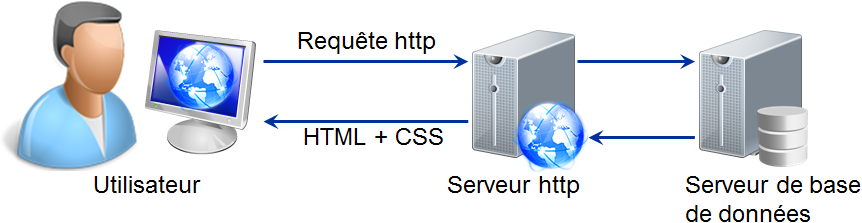
\includegraphics[scale=0.5]{../graph/protocoleHTTP.png} \\
  \caption{Protocole HTTP - \url{https://aresu.dsi.cnrs.fr/spip.php?article137}}
\end{figure}
Un navigateur ne fait rien d'autre que traduire/interpréter des informations qui lui sont envoyées sous forme HTML, CSS et Javascript. Le serveur ne devra donc renvoyer des informations qu'à l'aide de ces technologies.
De même, le serveur de son côté utilise des technologies propres à lui qui lui permettent d'analyser les données reçues, de les transformer, de les enregistrer dans une base de données, etc... Finalement, il doit générer des pages web à envoyer au client après avoir réaliser les traitements nécessaires.\\

D'autres technologies que Java EE permettent de traiter les informations sur le serveur comme PHP, .NET ou encore Django, mais nous avons préférer utiliser un environnement connu et déjà utilisé lors d'autres projets. Ainsi nous avons pu gagner un peu de temps et nous pencher sur d'autres problématiques. De plus, nous souhaitions utiliser le langage Java et cette technologie nous le permet.

Un avantage de Java EE est qu'il a été créé notamment pour faciliter le travail en équie sur un même projet. En effet, l'application est formée de plusieurs couches.

\subsubsection{Mise en place sous Eclipse}
Pour créer notre application web avec Java EE nous avons besoin d'un \textit{Environnement de Développement Intégré} (IDE) qui est un logiciel facilitant le développement de l'application. Nous avons choisi d'utiliser l'IDE Eclipse qui nous était déjà familier et car il est gratuit, puissant, libre et multiplateforme.\\
Un tel logiciel a différents avantages comme par exemple :
\begin{itemize}
 \item Une interface graphique avec une hiérarchie permettant de visualiser l'architecture de l'application
 \item L'intégration des outils nécessaires au développement de l'application.
 \item La possibilité de paramétrer facilement les composants de l'application.
 \item L'aide à l'écriture du code et même la génération automatique de certaines fonctions (exemple : les getters et setters).
 \item Un outil pour déboguer facilement.
\end{itemize}

On utilise donc la version d'Eclipse adéquate disponible sur le site officiel :
\begin{figure}[H]
  \center
  
\includegraphics[scale=0.5]{../graph/eclipse.png} \\
  \caption{Eclipse IDE for Java EE Developers - \url{https://eclipse.org/downloads/}}
\end{figure}

Une fois qu'Eclipse est installé, il est nécessaire de mettre en place un serveur d'applications. Nous avons utilisé Tomcat car il est libre, gratuit, multiplateforme et léger. Il est suffisant pour notre application.

\paragraph{Le serveur Apache Tomcat}
Apache Tomcat est un conteneur web libre de servlets et JSP Java EE. Nous verrons dans les parties suivantes ce que sont les servlets et les JSP. Il permet notammement l'utilisation des servlets et des JSP (JavaServer Pages).
Tomcat est un serveur HTTP avant tout. Il est écrit en Java ce qui permet de l'utiliser sur n'importe quelle système d'exploitation via la machine virtuelle Java.
\begin{figure}[H]
  \center
  
\includegraphics[scale=0.25]{../graph/apache.png} \\
  \caption{Apache Tomcat - \url{http://tomcat.apache.org/index.html}}
\end{figure}
En réalité, ce n'est pas un vrai serveur d'application mais un serveur web assemblé à un conteneur web. Dans notre projet, nous utilisons la dernière version d'Apache Tomcat 8.0 qui est suport de Java 7 et possède d'autres avantages dont nous avons besoin.

\paragraph{Dynamic Web Project}
Maintenant que le serveur Tomcat est ajouté, on peut créer le projet dans Eclipse. On crée un Dynamic Web Projet qui nous permettra de faire notre application.
Le schéma suivant donne la structure des fichiers de notre dossier projet :\\
\begin{figure}[H]
  \center
  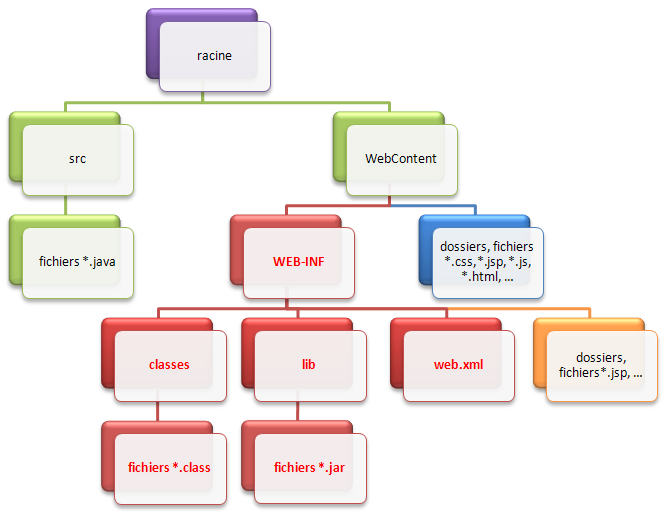
\includegraphics[scale=0.5]{../graph/schemaProjetDynamic.png} \\
  \caption{Structure des fichiers d'une application web JSP/Servlet sous Eclipse (Java EE) - \url{https://openclassrooms.com/courses/creez-votre-application-web-avec-java-ee/outils-et-environnement-de-developpement}}
\end{figure}
Quelques remarques sur le schéma précédent :
\begin{itemize}
 \item Le dossier src : c'est ici que se trouvent les packages Java et notamment les packages du modèle et du contrôleur.
 \item Le dossier WEB-INF : il est spécial et essentiel au bon fonctionnement de l'application. Il contient le fichier web.xml qui configure l'application, un dossier nommé classes qui contient les classes Java compilées et un dossier lib contenant les bibliothèques supplémentaires (.jar). Cette structure du dossier WEB-INF doit impérativement être comme ci-dessus.
 \item Les fichiers et dossiers publics sont placés dans le WebContent (en bleu) et les privés dans le WEB-INF. Cette notion de public/privé servira notamment lorsque l'on voudra bloquer l'accès à certaines pages.
 \item Le dossier WebContent est propre à Eclipse et n'est pas un dossier nécessaire à l'origine.
\end{itemize}
Enfin, il est important de préciser que si l'application n'est pas strucutrée de cette manière alors le serveur d'applications ne sera pas capable de la déployer et ainsi elle ne pourra pas fonctionner correctement.\\


Le projet est maitenant ouvert et il est alors possible de créer une première page web. Si l'on voulait créer une simple page web statique il suffirait de créer une fichier HTML dans le dossier WebContent. Pour créer des pages dynamiques on va avoir recours aux servlets et aux Java Server Pages décrites dans ce qui suit.


\subsubsection{Les servlets}
Les servlets sont des classes implémentées en Java qui permettent de rendre dynamique une page HTML. Elles utilisent l'API Java Servlet qui correspond au package javax.servlet.\\

Si on repart du schéma suivant, on reprend le mécanisme existant entre le client et le serveur HTTP : le client envoie une requête HTTP au serveur et ce dernier lui retourne une réponse.\\
\begin{figure}[H]
  \center
  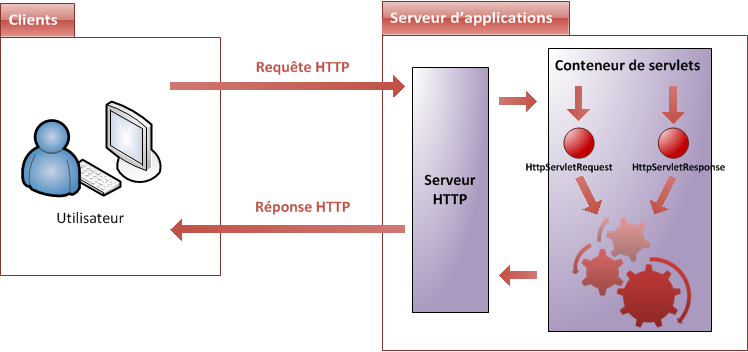
\includegraphics[scale=0.5]{../graph/serveurclient.png} \\
  \caption{Schéma serveur client et protocole HTTP - \url{https://openclassrooms.com/courses/creez-votre-application-web-avec-java-ee/la-servlet}}
\end{figure}

Tout l'intérêt de l'utilisation des servlets réside dans le fait qu'il devient alors possible de maîtriser le traitement des requêtes mais surtout de personnaliser les réponses HTTP qui sont faites au client.\\
Ainsi, dans la plupart des cas, le fonctionnement d'une servlet peut se résumer au fait que c'est une classe Java qui reçoit une requête HTTP envoyée depuis un navigateur par un client et lui renvoie une réponse HTTP.\\
L'ensemble des servlets est appelé conteneur de servlets ou conteneur web et c'est Apache Tomcat qui les gère.

\paragraph{Implémentation}
Lors de l'implémentation d'une servlet en Java, il faut créer une classe qui hérite de la classe abstraite HttpServlet et pour cette raison elle doit implémenter à
minima l'un des trois méthodes suivantes :
\begin{itemize}
 \item doGet() : gère la méthode GET et est appelée à l'ouverture de la page web.
 \item doPost() : gère la méthode POST et est appelée suit à la validation d'un formulaire généralement.
 \item doHead() : gère la méthode HEAD qui est proche de GET mais ne renvoie que les en-têtes HTTP.
\end{itemize}
Il faut ensuite déclarer à notre application l'existence de la servlet. Pour cela on a le ficher de configuration web.xml. Ainsi, il faudra préciser à ce fichier la définition de chaque nouvelle servlet.
On prend comme exemple une servlet JoueurServlet.java qu'on aura pris soin de placer dans le package controleur (dans le dossier src). Dans le fichier web.xml on a deux étapes :
\begin{enumerate}
 \item Déclaration de la servlet : on la nomme et on précise son emplacement dans le projet.
\begin{lstlisting}
  <servlet>
    <servlet-name>JoueurServlet</servlet-name>
    <servlet-class>controleur.JoueurServlet</servlet-class>
  </servlet>
\end{lstlisting}  
 \item Correspondance de la servlet avec une URL (le mapping) : on défini l'URL associée à la servlet, le nom doit être le même que celui défini ci-dessus.
\begin{lstlisting}
  <servlet-mapping>
    <servlet-name>JoueurServlet</servlet-name>
    <url-pattern>/joueur</url-pattern>
  </servlet-mapping>
\end{lstlisting}  
\end{enumerate}

En général, on met dans la méthode doGet les éléments qui seront affichés au démarrage de la page. On peut écrire le code HTML dans la fonction \textit{out.println()} mais on préférera utiliser les JSP définies dans ce qui suit. La méthode doPost sera elle appelée par l'utilisateur lors de la saisie d'un formulaire par exemple. On récupérera les informations saisies par l'utilisateur avec la méthode \textit{getParameter('nom du paramètre')}.
Des méthodes et classes du package modèle pourront être appelées ici. A la fin des méthodes il faudra faire un forward des données vers la JSP correspondante.\\

Les servlets sont mises dans le package contrôleur qui sera donc la partie contrôleur de l'architecture MVC.

\subsubsection{Les JSP (Java Server Pages)}
Une Java Server Page (on utilisera le terme de JSP par la suite) est un document texte qui peut contenir des balises HTML mais également des balises permettant d'inclure du code Java. Le langage utilisé dans les JSP permet aussi l'utilisation d'autres technologies comme XML, les servlets, le CSS, le JavaScript... et ce dans un seul et unique fichier ce qui rend les rend d'autant plus intéressantes.\\

On utilise des JSP car cela simplifie l'utilisation des technologies servlets. En effet, écrire une page web en Java peut vite devenir pénible. Les JSP permettent donc d'utiliser la technologie des servlet d'une manière simplifiée puisqu'on peut écrire une page HTML de manière classique.\\

D'autre part, on les utilise afin de respecter la structure MVC puisque cela permet de retirer des servlets la partie 'vue' et de n'y laisser que la partie 'contrôleur'. De même on sépare la vue du modèle puisque il peut se trouver au milieu des servlets du code métier. Ainsi, la servlet est le contrôleur qui relie la vue (JSP) au modèle. Tout ceci respectant bien l'architecture MVC.\\

L'avantage de l'utilisation des JSP est que les pages sont exécutées par un serveur et ainsi on peut avoir une page dynamique contrairement aux pages HTML basiques.\\

La page étant alors dynamique, on peut faire varier l'affichage de la page et avoir une interaction avec l'utilisateur.\\

Si l'on fait un formulaire dans la JSP (formulaire HTML), on lui affectera la méthode POST et ainsi la méthode doPost de la servlet correspondante sera activée et l'affichage sera modifiée en fonction du contenu de la méthode doPost. On peut par exemple changer de page si la servlet redirige vers une autre page. C'est par exemple le cas lors de la connexion d'un utilisateur à un site web : il saisi sont login et son mot de passe, valide le formulaire et, s'il a bien saisi ses informations, la servlet l'aura vérifié et le redirigera vers une autre page.\\

Les JSP sont donc la partie vue du modèle MVC puisqu'elles correspondent aux pages web avec lesquelles l'utilisateur interagi.

\subsubsection{Application de l'architecture MVC à l'exemple d'un Joueur}
Dans cet exemple on considère que l'utilisateur est sur une page web intitulée générée par la JSP Joueur.jsp. Il rempli un formulaire quelconque par exemple pour moddifier son âge. La servlet reçoit un message et sa méthode doPost est déclenchée. Au sein de sa méthode doPost elle fait appelle au modèle, la classe Joueur.java, et plus précisemment la méthode qui modifie l'âge (setAge par exemple). L'âge est alors modifié dans le modèle, ce dernier renvoie à la servlet le nouvel âge et lui signifie que la modification a été effectuée. Enfin, la servlet forward vers la page web le nouvel âge du joueur.
\begin{figure}[H]
  \center
  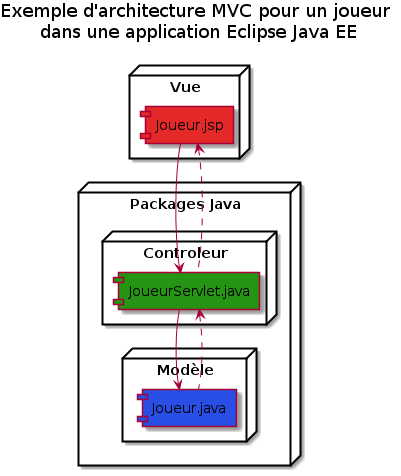
\includegraphics[scale=0.5]{../graph/exempleMVC.png} \\
  \caption{Exemple d'application de la structure MVC à notre environnement Java EE}
\end{figure}
